\documentclass[12pt]{article}\usepackage[]{graphicx}\usepackage[]{color}
%% maxwidth is the original width if it is less than linewidth
%% otherwise use linewidth (to make sure the graphics do not exceed the margin)
\makeatletter
\def\maxwidth{ %
  \ifdim\Gin@nat@width>\linewidth
    \linewidth
  \else
    \Gin@nat@width
  \fi
}
\makeatother

\definecolor{fgcolor}{rgb}{0.345, 0.345, 0.345}
\newcommand{\hlnum}[1]{\textcolor[rgb]{0.686,0.059,0.569}{#1}}%
\newcommand{\hlstr}[1]{\textcolor[rgb]{0.192,0.494,0.8}{#1}}%
\newcommand{\hlcom}[1]{\textcolor[rgb]{0.678,0.584,0.686}{\textit{#1}}}%
\newcommand{\hlopt}[1]{\textcolor[rgb]{0,0,0}{#1}}%
\newcommand{\hlstd}[1]{\textcolor[rgb]{0.345,0.345,0.345}{#1}}%
\newcommand{\hlkwa}[1]{\textcolor[rgb]{0.161,0.373,0.58}{\textbf{#1}}}%
\newcommand{\hlkwb}[1]{\textcolor[rgb]{0.69,0.353,0.396}{#1}}%
\newcommand{\hlkwc}[1]{\textcolor[rgb]{0.333,0.667,0.333}{#1}}%
\newcommand{\hlkwd}[1]{\textcolor[rgb]{0.737,0.353,0.396}{\textbf{#1}}}%

\usepackage{framed}
\makeatletter
\newenvironment{kframe}{%
 \def\at@end@of@kframe{}%
 \ifinner\ifhmode%
  \def\at@end@of@kframe{\end{minipage}}%
  \begin{minipage}{\columnwidth}%
 \fi\fi%
 \def\FrameCommand##1{\hskip\@totalleftmargin \hskip-\fboxsep
 \colorbox{shadecolor}{##1}\hskip-\fboxsep
     % There is no \\@totalrightmargin, so:
     \hskip-\linewidth \hskip-\@totalleftmargin \hskip\columnwidth}%
 \MakeFramed {\advance\hsize-\width
   \@totalleftmargin\z@ \linewidth\hsize
   \@setminipage}}%
 {\par\unskip\endMakeFramed%
 \at@end@of@kframe}
\makeatother

\definecolor{shadecolor}{rgb}{.97, .97, .97}
\definecolor{messagecolor}{rgb}{0, 0, 0}
\definecolor{warningcolor}{rgb}{1, 0, 1}
\definecolor{errorcolor}{rgb}{1, 0, 0}
\newenvironment{knitrout}{}{} % an empty environment to be redefined in TeX

\usepackage{alltt}

\usepackage[utf8]{inputenc}
\usepackage[T1]{fontenc}
\usepackage[french]{babel}
\usepackage[hidelinks]{hyperref}
\usepackage{amsmath}
%\usepackage{fullpage}
\usepackage{microtype}
\usepackage[backend=biber]{biblatex}
\usepackage{float}
\usepackage{csquotes}

\title{Étude de marché de la Citroën Cactus}
\author{Marc \textsc{Autrand}, Timothée \textsc{Pallot}, Edouard
	\textsc{Nguon}, Rémi \textsc{Nicole}}
\date{11 décembre 2015}

\addbibresource{liography.bib}
\IfFileExists{upquote.sty}{\usepackage{upquote}}{}
\begin{document}

\maketitle

\tableofcontents

\part{Pré-enquête}

\section{Introduction}

\paragraph{} Dans le cadre de l'unité MSH-3001, nous avons réalisé une étude
sur les marques Citroën, et notamment la C4 Cactus et DS. Carlos Tavarez nous a
demandé de le conseiller dans sa stratégie marketing.

\paragraph{} Nous avons donc sondé une centaine de personnes afin de connaître
leur avis sur la C4 Cactus: son design, ses fonctionnalités, la stratégie de
Citroën en créant une voiture totalement différente de sa production
habituelle. Nous avons aussi obtenu leurs avis sur la marque DS, son design
comparé à des marques de luxe comme Audi et les conséquences de la séparation
avec la marque Citroën sur cette dernière.

\paragraph{} Nous avons aussi réussi a discuter avec deux conseillers
commerciaux de Renault et Peugeot, contrairement à des concessionnaires comme
Citroën (pour l'instant) et Toyota qui n'ont pas trouvé le temps de nous
répondre du fait de la forte présence de clients.

\section{Historique}

\paragraph{} L'histoire récente de PSA Peugeot-Citroën est marquée par
plusieurs bouleversements. Depuis le rachat de Citroën à Michelin en 1976, le
groupe doit relever le défi de faire cohabiter deux marques concurrentes. Si la
distinction claire entre les clients Citroën et Peugeot, creusée depuis les
années 1950, semblait être un avantage, le groupe parvint difficilement à
concilier les différences de culture et d'approche des deux constructeurs. Peu
à peu, il s'éloigne du marché haut de gamme, duquel Citroën était pourtant
proche.

\paragraph{} En 2009, le lancement de la gamme DS ouvre de nouveaux horizons.
Créé par le PDG sortant Christian Streiff, le label mise sur le retour très
populaire des anciens modèles phares des marques européennes : Mini Cooper,
Fiat 500, etc\ldots Si le sigle DS apporte l'héritage de la gamme mythique des
années 1960, le design est celui d'une marque premium, tout comme le prix des
modèles. Citroën part ainsi à l'assaut de ténors comme Audi, mais aussi du
marché chinois, longtemps délaissé, pour lequel le prix a moins d'importance
que la qualité du véhicule.

\paragraph{} La ligne DS est un succès. Pour autant, sa communication l'éloigne
de Citroën ; puis, en 2014, le groupe PSA choisit d'en faire une filiale à part
entière. Ne reste alors plus à Citroën que sa seconde spécialité, celle de
faire du différent. Elle présente ainsi au même moment un modèle d'un genre
nouveau, entre la berline et le SUV, et doté d'un design particulier : la C4
Cactus, première d'une génération de voitures vouée à redéfinir la gamme
Citroën.

\paragraph{} Si la stratégie du groupe PSA depuis 2014 a été efficace, en
renouant dès le premier semestre 2015 avec les bénéfices\cite{lesechos}, le
futur est plus incertain. La C4 Cactus est un modèle clivant qui rassemble de
nombreux fans mais souffre d'un manque de reconnaissance du grand public. La
gamme DS, quant à elle, prend son envol en Chine et devient le porte-étendard
du groupe.\\

\noindent \emph{Quel développement peuvent connaître ces deux gammes, et
	peuvent-elles coexister?}

\section{Méthodologie}

\paragraph{} Afin de réaliser notre étude, nous sommes allés rencontrer des
concessionnaires comme Peugeot et Renault afin d'avoir l'avis personnel de
conseillers commerciaux. Pour élargir notre champ de recherche, nous avons
aussi créé un sondage qui nous avons fait passer dans des réseaux sociaux comme
Facebook afin d'avoir des avis divers et variés venant de catégories de
personnes différentes.

\paragraph{} Le positionnement de la Cactus, proche des SUV, lui donnant plus
de chances de trouver un public à l'étranger qu'en France, nous avons également
cherché des retours à l'international. Cette décision était confortée par les
prix reçus par le véhicule : voiture de l'année en Espagne et au Danemark, prix
du design de New York, etc\ldots Nous avons ainsi réalisé une version du
sondage en langue anglaise, afin de la partager sur les réseaux sociaux mais
aussi auprès de communautés d'amateurs de voitures françaises. Si une majorité
de retours nous sont venus du Royaume-Uni, des réponses ont aussi été données
depuis le Brésil, la Turquie et plusieurs pays européens.\\

\noindent Le total de personnes interrogées s'élève à plus de 130.

\part{Résultats}

\section{Retour des échanges avec les concessionnaires}

\paragraph{} Nous avons pu interroger deux conseillers commerciaux des
concessionnaires Peugeot et Renault, le premier étant partenaire de Citroën dans
le groupe PSA, et le second un concurrent de la marque.

\paragraph{} Le conseiller de Renault nous a donné un avis plutôt négatif
concernant la C4 Cactus. Il travaille à Renault, mais ne se considère pas comme
fidèle à Renault, ce qui nous a permis d'avoir un avis plutôt subjectif de la
part d'un homme ayant certainement la vingtaine. Il n'est pas du tout satisfait
du design de la C4 Cactus, trouvant les air-bumps disgracieux et pas efficaces.
En effet cette personne a travaillé dans la production des voitures avant de
s'engager dans le commercial et a vu beaucoup de Citroën C4 Cactus revenir au
garage à cause des air-bumps car lorsque ceux-ci sont abîmés et doivent être
changés, il faut changer les deux portes étant reliées à l'air-bump cassé et
tout le plastique autour, ce qui demande beaucoup de temps et de main d'œuvre.
De plus, de son point de vue, la partie avant de la voiture ressemble trop à
celle d'un 4x4, elle est trop imposante ce qui ne correspond pas à ce que
produit Citroën habituellement.

\paragraph{} En ce qui concerne la marque DS, son avis est totalement
différent. Pour lui, le design des voitures de la marque est très beau
esthétiquement et la nouvelle marque a eu la bonne idée de se séparer de
Citroën. Cependant, les prix affichés par DS sont trop élevés pour prétendre
atteindre des ventes aussi importantes que ses concurrents.

\paragraph{} Le conseiller commercial de Peugeot que nous avons interrogé a lui
aussi un avis très négatif sur la C4 Cactus. Le design de cette voiture est
beaucoup trop décalée par rapport à ce que fabrique généralement la marque. La
technologie air-bump, notamment, n'est pas du tout du goût de conseiller qui ne
la trouve absolument pas exceptionnelle malgré tout le bourrage médiatique fait
par la marque autour de celle-ci.

\paragraph{} Pour ce qui est de la marque DS, elle a fabriqué de très bons
produits comme la DS3 et la DS4, mais celui-ci se rapproche beaucoup trop de la
Citroën C4: si on ne regarde pas les phares, les deux voitures sont identiques.
Pour lui, la marque DS a plusieurs gros problèmes: le premier est que les
premières DS et notamment les plus médiatisées DS3 et DS4 ont été vendues par
Citroën, et non par DS. Le deuxième problème de la marque est sa politique de
prix: elle fournit des voitures à prix élevés de l'ordre de ceux des véhicules
produits par Audi ou BMW, mais pas de la même qualité.

\paragraph{} De plus, Citroën a voulu aller trop vite car à l'origine, la
marque produisait des voitures qui n'étaient pas adapté au public des jeunes
personnes.  Elle ne produit pas non plus de voitures de luxe, et n'était pas
assez reconnue pour avoir l'effet escompté sur le grand public. Elle a voulu
être en avance sur son temps, mais s'est essoufflée. Par exemple, pour la
Peugeot 3008, les ingénieurs de la marque ont conçus cette voiture en 2009,
mais la voiture n'a été fabriquée que 4 ans plus tard. Il ont eu la présence
d'esprit d'avoir anticipé le futur besoin des gens en avance de 4 ans et de la
commercialiser au bon moment.

\paragraph{} Enfin, le dernier problème de DS se situe dans ses garages: ils
n'ont pas misés leurs efforts sur la qualité, ce qui n'est pas respectueux de
la part d'un constructeur de voitures de luxe dont les prix sont de l'ordre de
50 000 voire 70 000 €.

\section{État des ventes de la Cactus et de DS, publics concernés}

\subsection{Citroën C4 Cactus}

\paragraph{} Avec sa mise en vente en 2014, la C4 Cactus connaît un début
discret en terme de vente mais a réussi tout de même à enregistrer 75 000
ventes au bout d'un an ainsi que 35 distinctions à travers le
monde\cite{communique}, mais seulement 27\% ont été vendues en France. Les
Français sont beaucoup moins attirés par ce modèle car le modèle n'a pas été
commandé plus de 20 000 fois depuis son lancement en Juin 2014 et a été vendus
en seulement 6 000 exemplaires en cette année 2015. Il faut aussi prendre en
compte le fait que les agents de la marque en ont presque tous une par
obligation et les concessionnaires en ont en stock donc ces chiffres ne sont
pas tout à fait révélateurs du nombre de clients qui en ont acheté une. De
plus, le modèle ne pointe qu'à la 22\ieme{} place des voitures les plus vendues
en France depuis le début de l'année 2015.

\paragraph{} Ce modèle allie confort et technologie utile et vise un public
cherchant plus un voiture utile qu'un voiture permettant d'affirmer son statut
social. En terme de prix, la Citroën Cactus se positionne entre voitures ``low
cost'' et voitures haut de gamme. En effet, son prix peut varier entre 15 200 €
et 22 900 € à neuf selon la finition et le moteur pris\cite{banquette}.

\subsection{Citroën DS}

\paragraph{} La marque DS s'est véritablement lancée avec la DS3 en 2010 qui a
été vendue en 26 417 exemplaires cette même année, 33 015 l'année suivante,
puis les ventes ont diminué avec 25 107 ventes en 2012 et 19 672 et 17 471
respectivement en 2013 et 2014. Ce modèle a plu à de nombreux clients de part
son design novateur\cite{avis}, son comportement routier exceptionnel, son
confort mais aussi son intérieur original et moderne. Les finitions sont
satisfaisantes, la voiture est très personnalisable, a une bonne habitabilité à
l'arrière et n'est pas très chère par rapport à ce que fait déjà Citroën,
puisqu'ils s'articulent autour de 20 000 € pour les modèles les plus chers.

\paragraph{} En revanche, elle a quelques défauts comme l'équipement qui n'est
pas très développé, la partie plastique qui n'est pas d'une grande qualités et
des bruits parasites viennent de temps en temps agacer le conducteur. Le
dernier point noir de ce modèle se situe au niveau des vitres arrières qui ne
peuvent pas s'ouvir. La DS4 viens s'ajouter au marché en 2011, soit un an après
la sortie de son ainée et elle ne suscite pas autant d'admiration chez les
clients car les ventes n'arrivent pas à décoller : 10 757 voitures vendues lors
de la première année, pour atteindre le pic de ventes l'année d'après avec 14
143 modèles vendus et retomber à 11 740 et 8 661 ventes en 2013 et 2014.

\paragraph{} La DS5 fait même moins de ventes que la DS4 puisque le nombre
maximum de voitures vendues sur une année est de 10 943 et concerne l'année de
sa sortie. Les deux année suivantes sont très mauvaises, pour ne pas dire
catastrophiques car les ventes tombent à 8 365 en 2013 et 5 614 en 2014. En
effet les défauts de la DS3 ne sont pas résolus sauf en ce qui concerne
l'équipement de la voiture. Le confort global est lui beaucoup moins bon sur la
DS4 et la DS5 que sur la DS3.

\paragraph{} Cette nouvelle marque se distingue beaucoup de Citroën dans son
design, son luxe mais aussi son prix. Elle ne touche plus le commun des mortels
(pas mal hein hihi, mais a changer peut etre), elle se rapproche plus des
marques allemandes telles que Audi et BMW. Elle touche donc plus les jeunes,
qui sont attirés par son style, son design, ses couleurs.

\break
\part{Analyse des résultats du sondage}

\section{Âge et sexe}



\begin{knitrout}
\definecolor{shadecolor}{rgb}{0.969, 0.969, 0.969}\color{fgcolor}\begin{figure}[H]
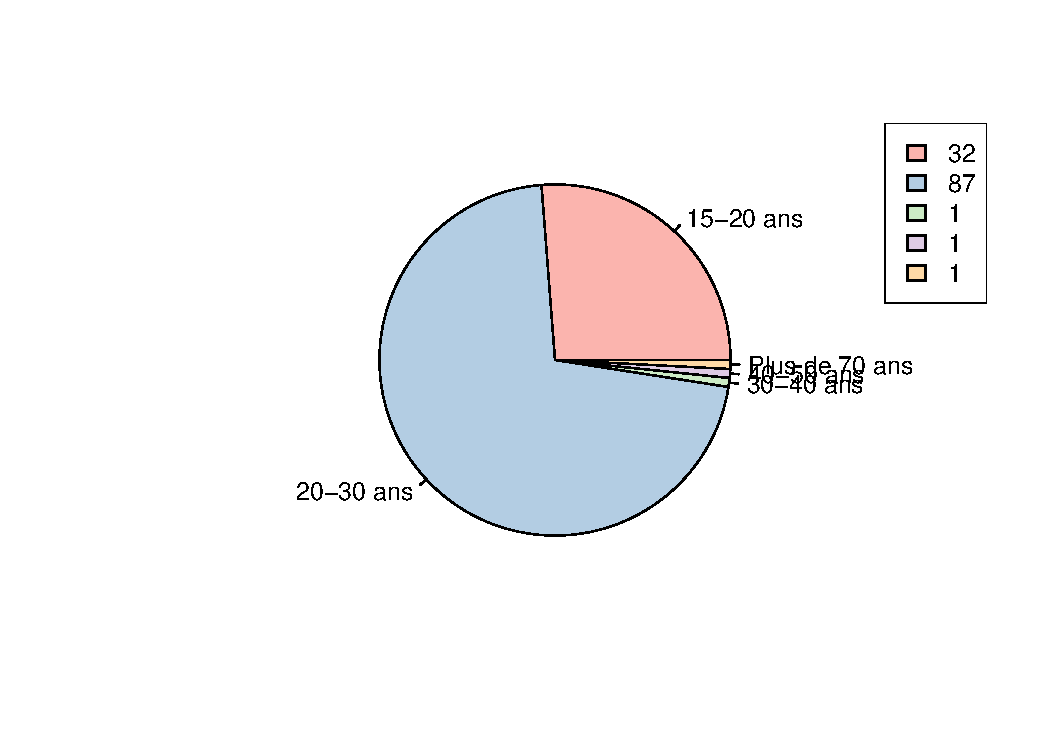
\includegraphics[width=\maxwidth]{figure/tranche_age_fr-1} \caption[Tranches d'âges des personnes ayant répondu au sondage français]{Tranches d'âges des personnes ayant répondu au sondage français}\label{fig:tranche age fr}
\end{figure}


\end{knitrout}

\begin{knitrout}
\definecolor{shadecolor}{rgb}{0.969, 0.969, 0.969}\color{fgcolor}\begin{figure}[H]
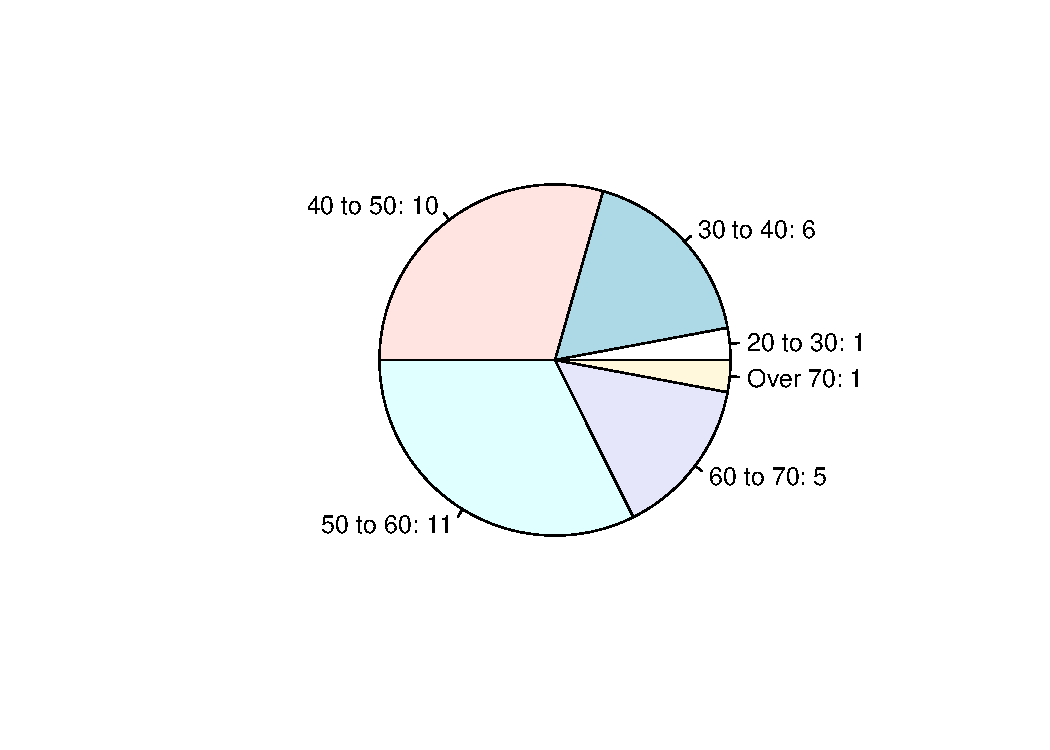
\includegraphics[width=\maxwidth]{figure/tranche_age_en-1} \caption[Tranches d'âges des personnes ayant répondu au sondage anglais]{Tranches d'âges des personnes ayant répondu au sondage anglais}\label{fig:tranche age en}
\end{figure}


\end{knitrout}

\begin{knitrout}
\definecolor{shadecolor}{rgb}{0.969, 0.969, 0.969}\color{fgcolor}\begin{figure}[H]
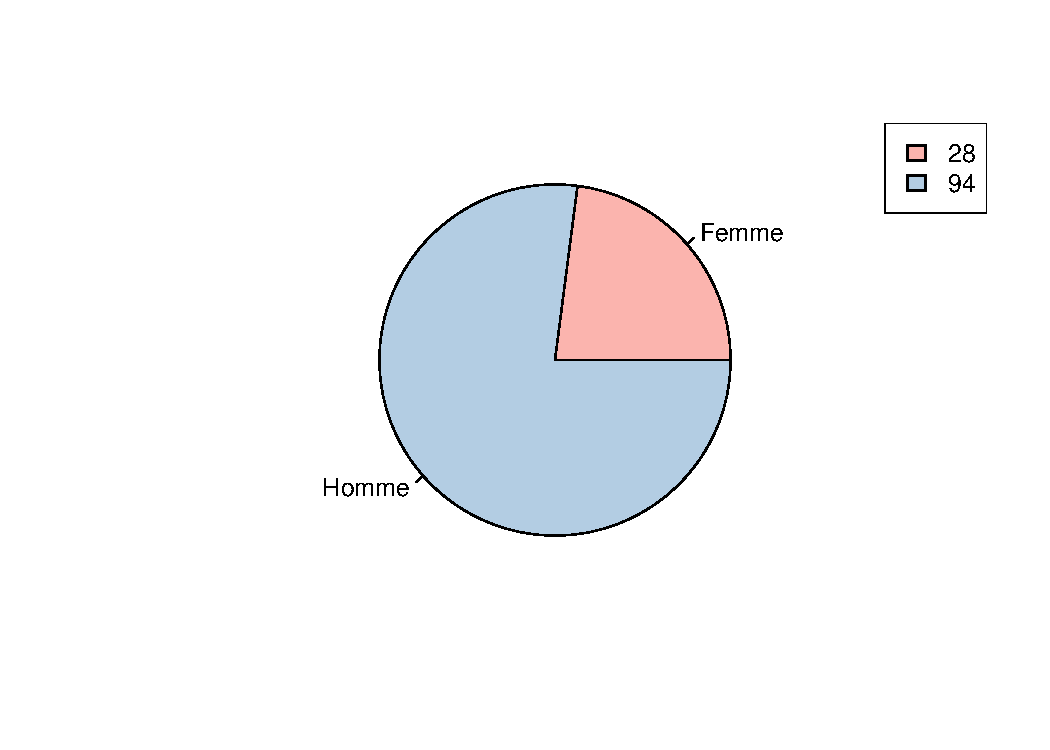
\includegraphics[width=\maxwidth]{figure/sexe_fr-1} \caption[Sexe des personnes ayant répondu au sondage français]{Sexe des personnes ayant répondu au sondage français}\label{fig:sexe fr}
\end{figure}


\end{knitrout}

\begin{knitrout}
\definecolor{shadecolor}{rgb}{0.969, 0.969, 0.969}\color{fgcolor}\begin{figure}[H]
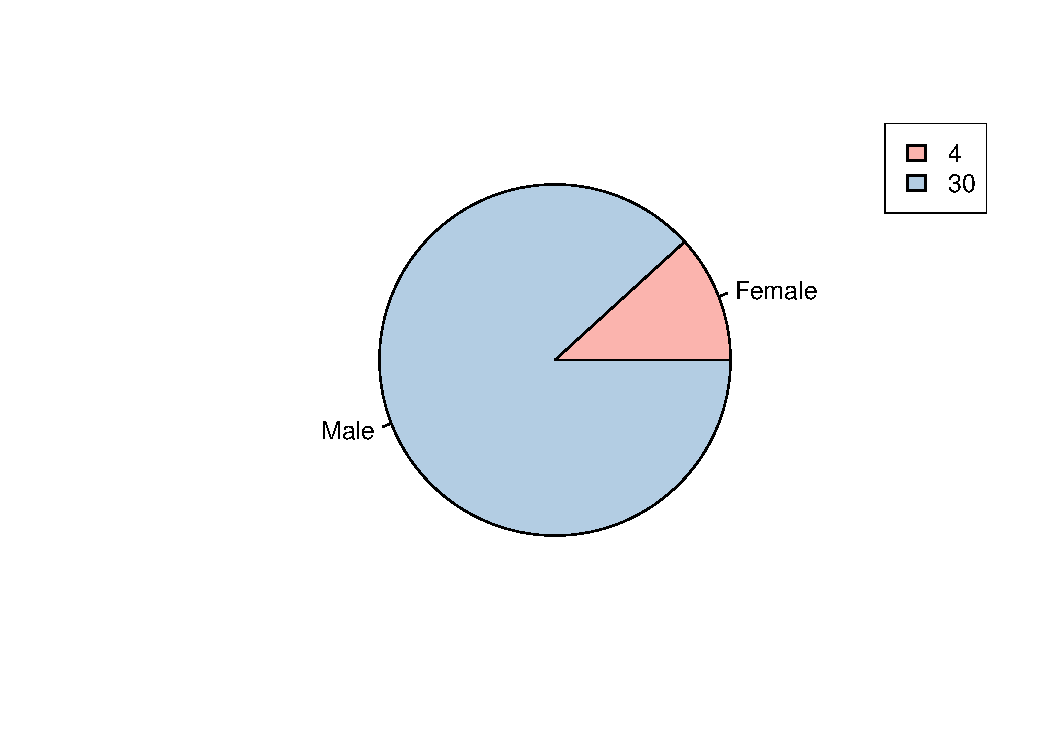
\includegraphics[width=\maxwidth]{figure/sexe_en-1} \caption[Sexe des personnes ayant répondu au sondage anglais]{Sexe des personnes ayant répondu au sondage anglais}\label{fig:sexe en}
\end{figure}


\end{knitrout}

\section{Marketing}

\begin{knitrout}
\definecolor{shadecolor}{rgb}{0.969, 0.969, 0.969}\color{fgcolor}\begin{figure}[H]
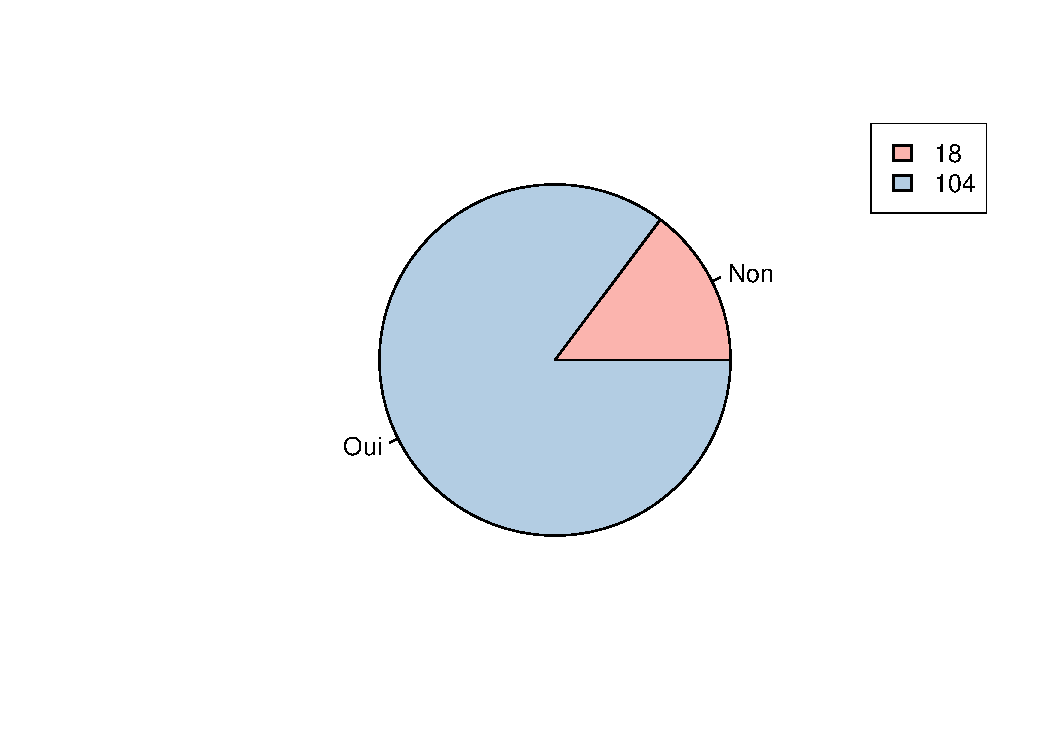
\includegraphics[width=\maxwidth]{figure/know_fr-1} \caption[Pourcentage des personnes connaissant auparavant la C4 Cactus ayant répondu au sondage français]{Pourcentage des personnes connaissant auparavant la C4 Cactus ayant répondu au sondage français}\label{fig:know fr}
\end{figure}


\end{knitrout}

\begin{knitrout}
\definecolor{shadecolor}{rgb}{0.969, 0.969, 0.969}\color{fgcolor}\begin{figure}[H]
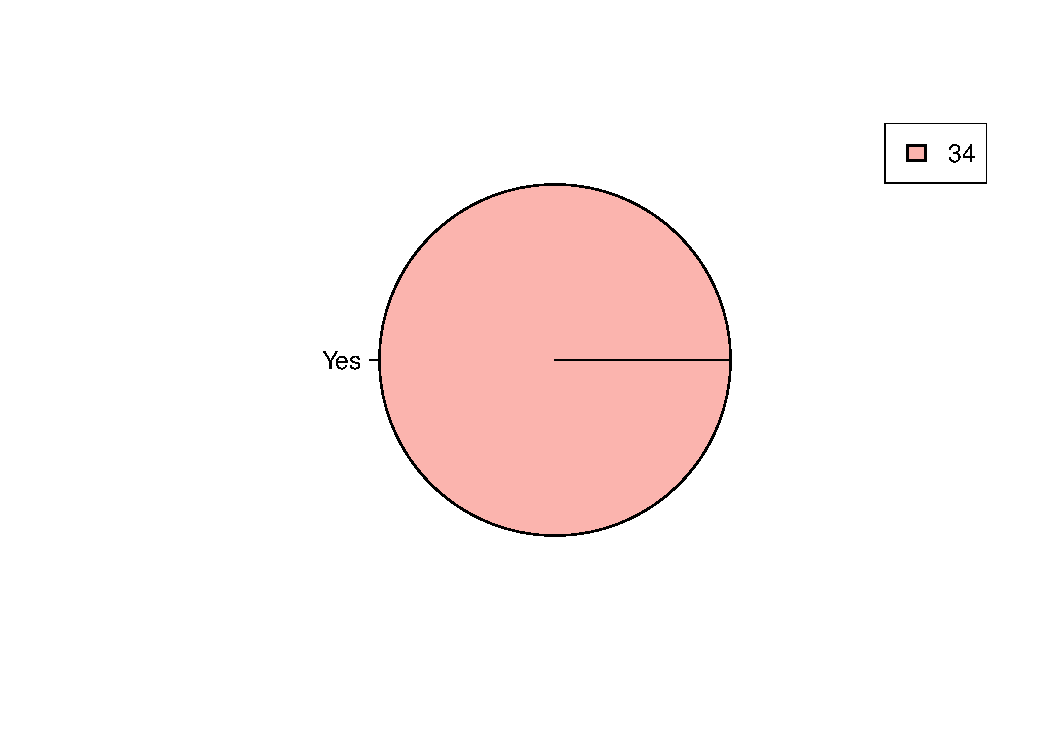
\includegraphics[width=\maxwidth]{figure/know_en-1} \caption[Pourcentage des personnes connaissant auparavant la C4 Cactus ayant répondu au sondage anglais]{Pourcentage des personnes connaissant auparavant la C4 Cactus ayant répondu au sondage anglais}\label{fig:know en}
\end{figure}


\end{knitrout}



\begin{knitrout}
\definecolor{shadecolor}{rgb}{0.969, 0.969, 0.969}\color{fgcolor}\begin{figure}[H]

\includegraphics[width=\maxwidth]{figure/means_fr-1} \caption[Nuage de mots du moyen de prise de conscience de l'existence de la C4 Cactus des personnes ayant répondu au sondage français]{Nuage de mots du moyen de prise de conscience de l'existence de la C4 Cactus des personnes ayant répondu au sondage français}\label{fig:means fr}
\end{figure}


\end{knitrout}

\begin{knitrout}
\definecolor{shadecolor}{rgb}{0.969, 0.969, 0.969}\color{fgcolor}\begin{figure}[H]
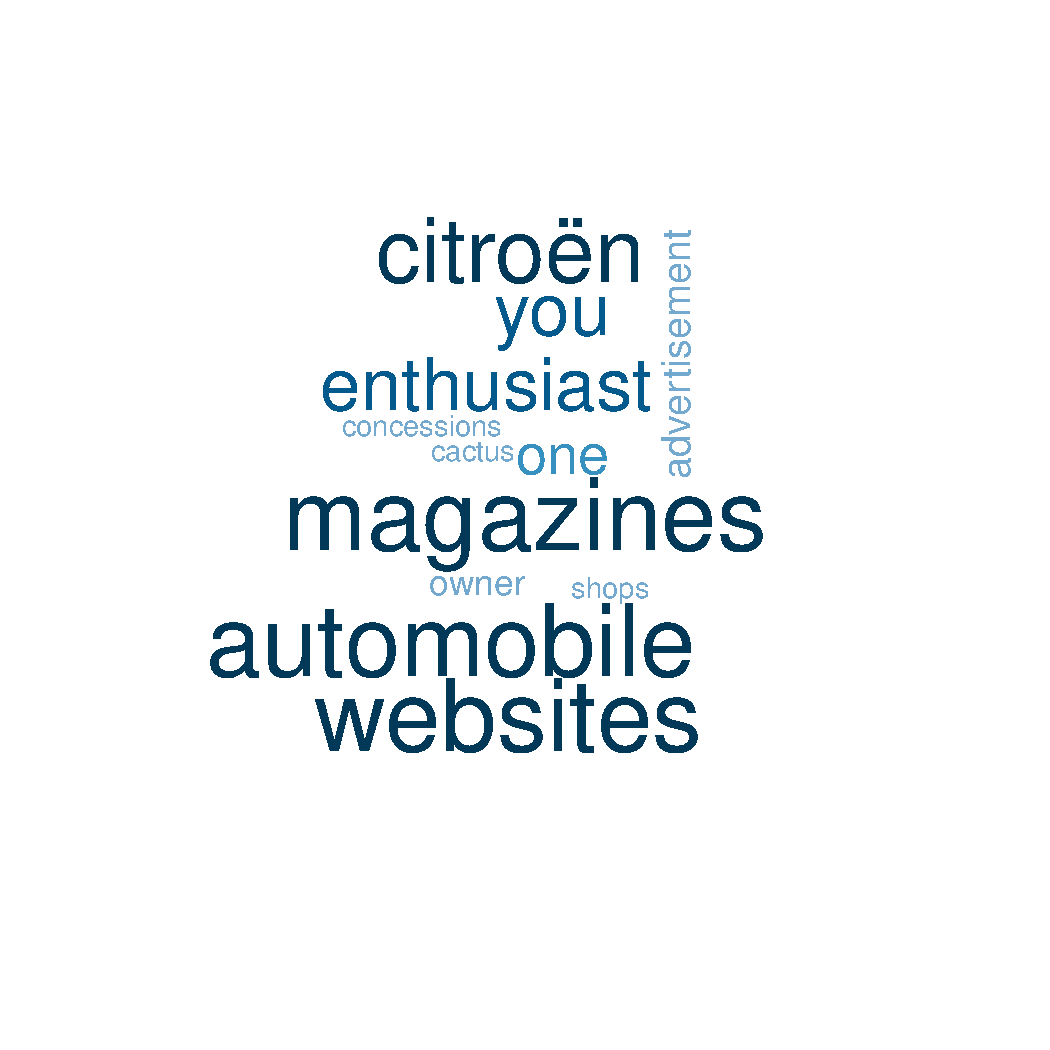
\includegraphics[width=\maxwidth]{figure/means_en-1} \caption[Nuage de mots du moyen de prise de conscience de l'existence de la C4 Cactus des personnes ayant répondu au sondage anglais]{Nuage de mots du moyen de prise de conscience de l'existence de la C4 Cactus des personnes ayant répondu au sondage anglais}\label{fig:means en}
\end{figure}


\end{knitrout}

\section{Apparence de la voiture}

\begin{knitrout}
\definecolor{shadecolor}{rgb}{0.969, 0.969, 0.969}\color{fgcolor}\begin{figure}[H]
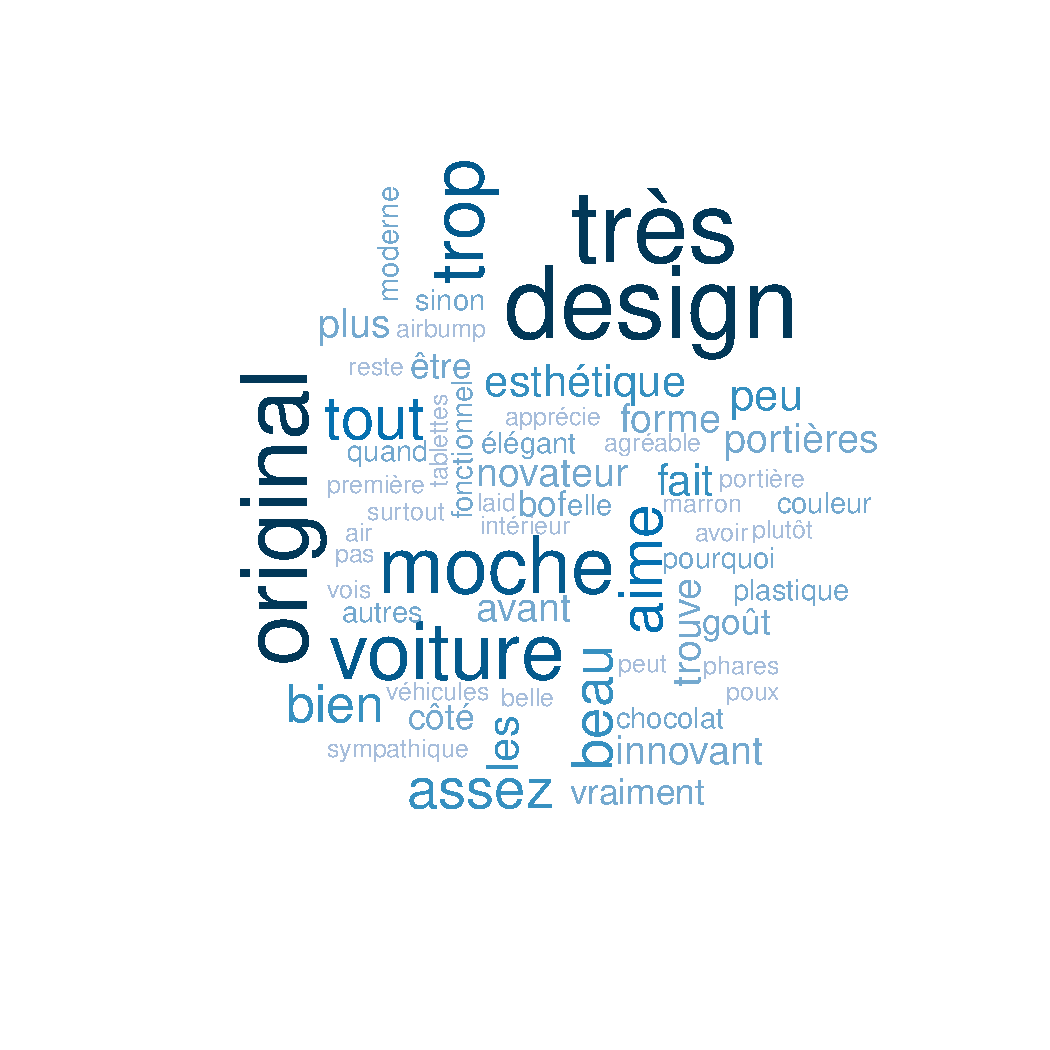
\includegraphics[width=\maxwidth]{figure/design_fr-1} \caption[Nuage de mots de l'avis du design de la C4 Cactus des personnes ayant répondu au sondage français]{Nuage de mots de l'avis du design de la C4 Cactus des personnes ayant répondu au sondage français}\label{fig:design fr}
\end{figure}


\end{knitrout}

\begin{knitrout}
\definecolor{shadecolor}{rgb}{0.969, 0.969, 0.969}\color{fgcolor}\begin{figure}[H]
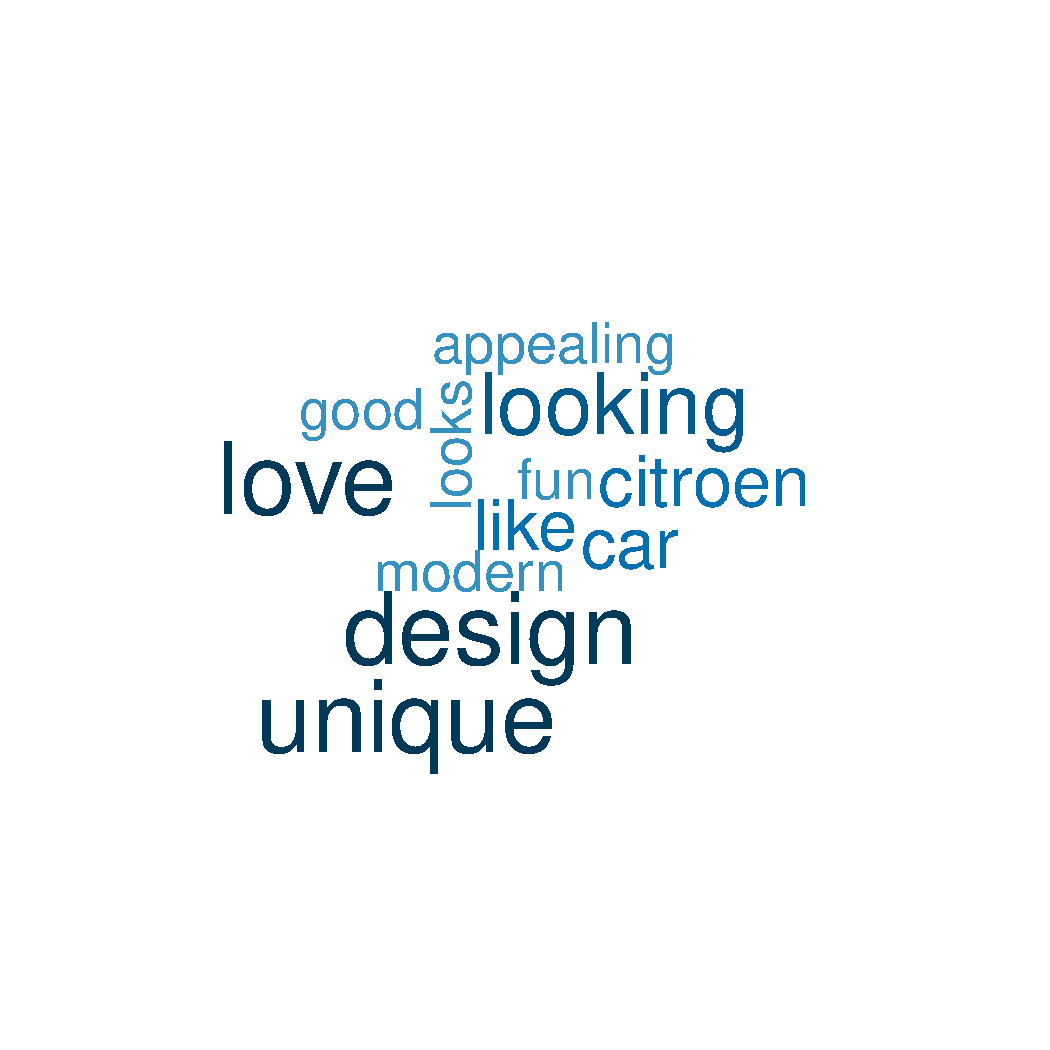
\includegraphics[width=\maxwidth]{figure/design_en-1} \caption[Nuage de mots de l'avis du design de la C4 Cactus des personnes ayant répondu au sondage anglais]{Nuage de mots de l'avis du design de la C4 Cactus des personnes ayant répondu au sondage anglais}\label{fig:design en}
\end{figure}


\end{knitrout}

\begin{knitrout}
\definecolor{shadecolor}{rgb}{0.969, 0.969, 0.969}\color{fgcolor}\begin{figure}[H]
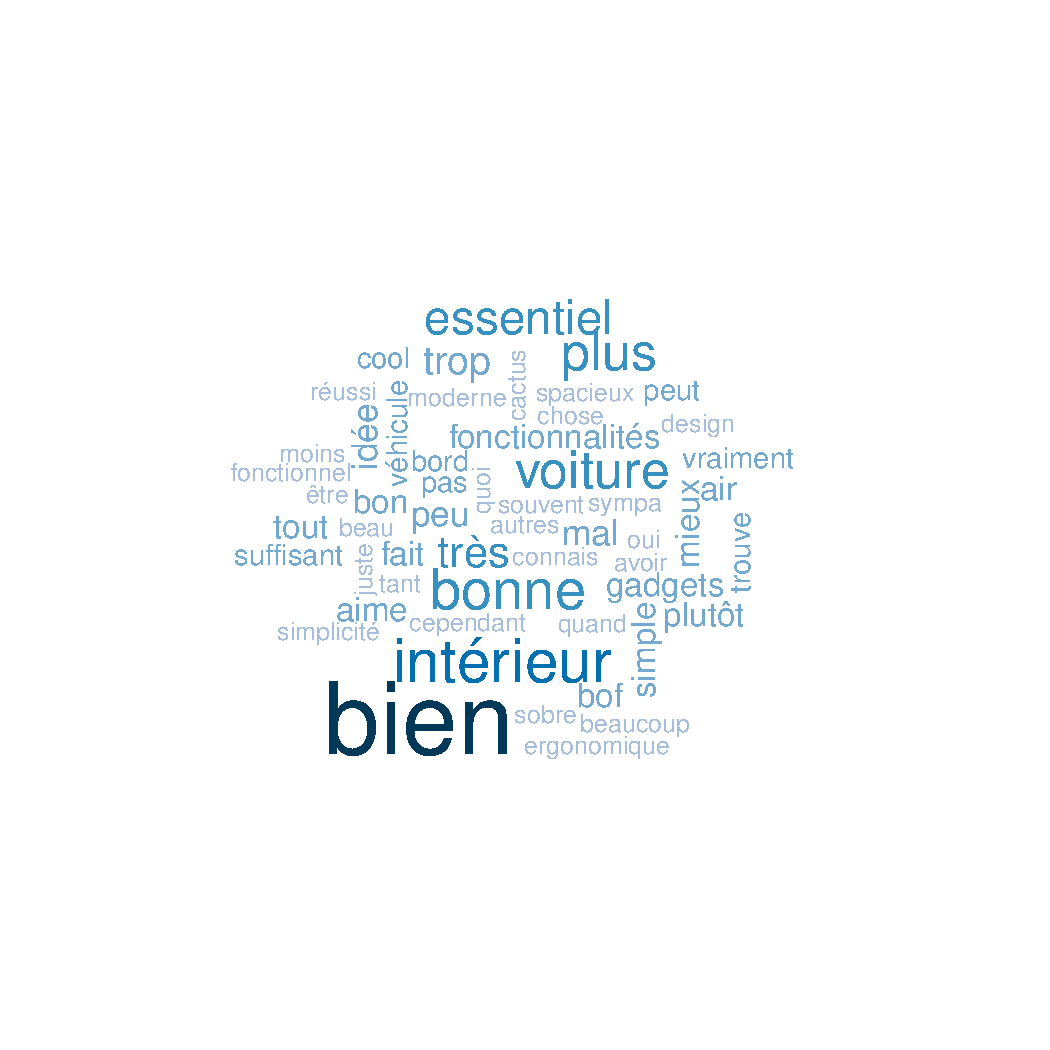
\includegraphics[width=\maxwidth]{figure/interior_fr-1} \caption[Nuage de mots de l'avis de l'intérieur de la C4 Cactus des personnes ayant répondu au sondage français]{Nuage de mots de l'avis de l'intérieur de la C4 Cactus des personnes ayant répondu au sondage français}\label{fig:interior fr}
\end{figure}


\end{knitrout}

\begin{knitrout}
\definecolor{shadecolor}{rgb}{0.969, 0.969, 0.969}\color{fgcolor}\begin{figure}[H]
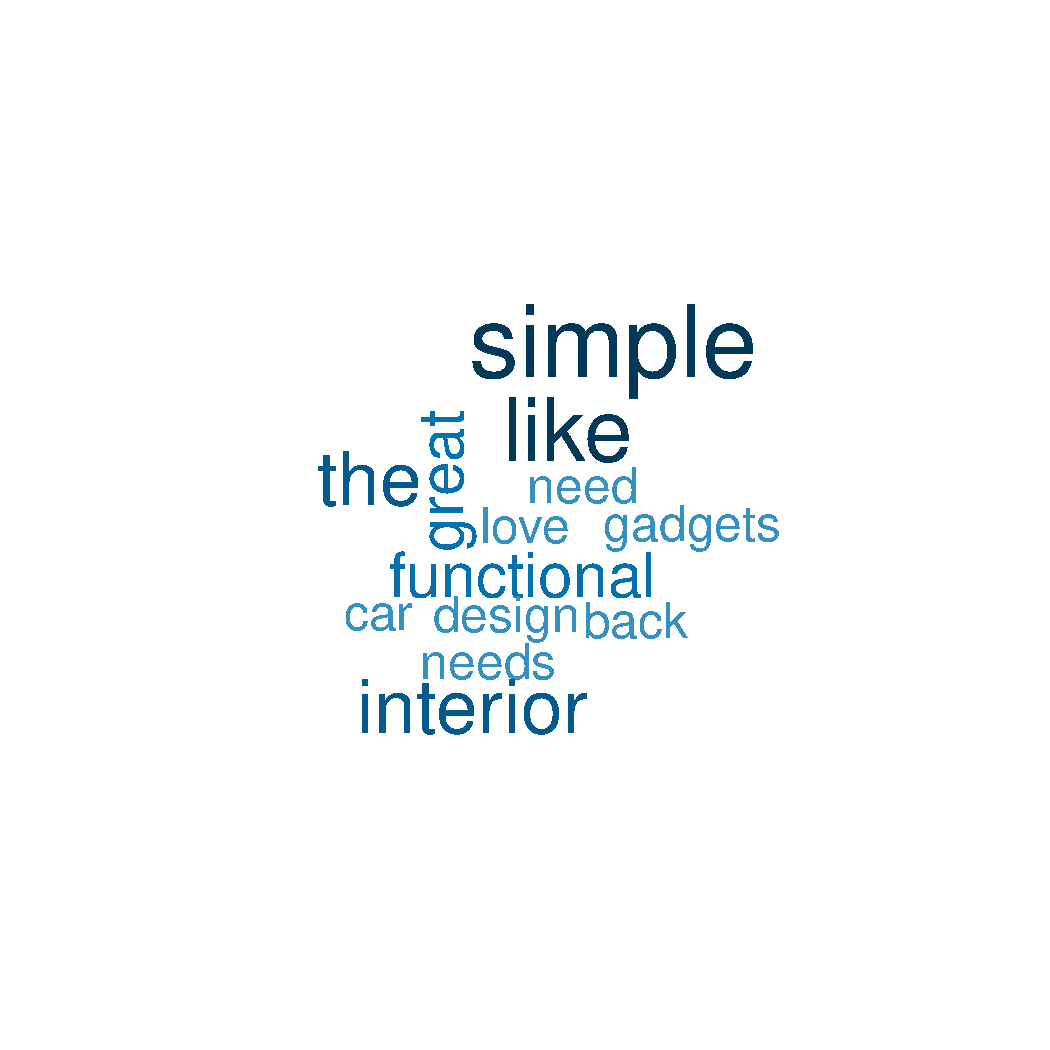
\includegraphics[width=\maxwidth]{figure/interior_en-1} \caption[Nuage de mots de l'avis de l'intérieur de la C4 Cactus des personnes ayant répondu au sondage anglais]{Nuage de mots de l'avis de l'intérieur de la C4 Cactus des personnes ayant répondu au sondage anglais}\label{fig:interior en}
\end{figure}


\end{knitrout}

\section{Opinion générale}



\begin{knitrout}
\definecolor{shadecolor}{rgb}{0.969, 0.969, 0.969}\color{fgcolor}\begin{figure}[H]
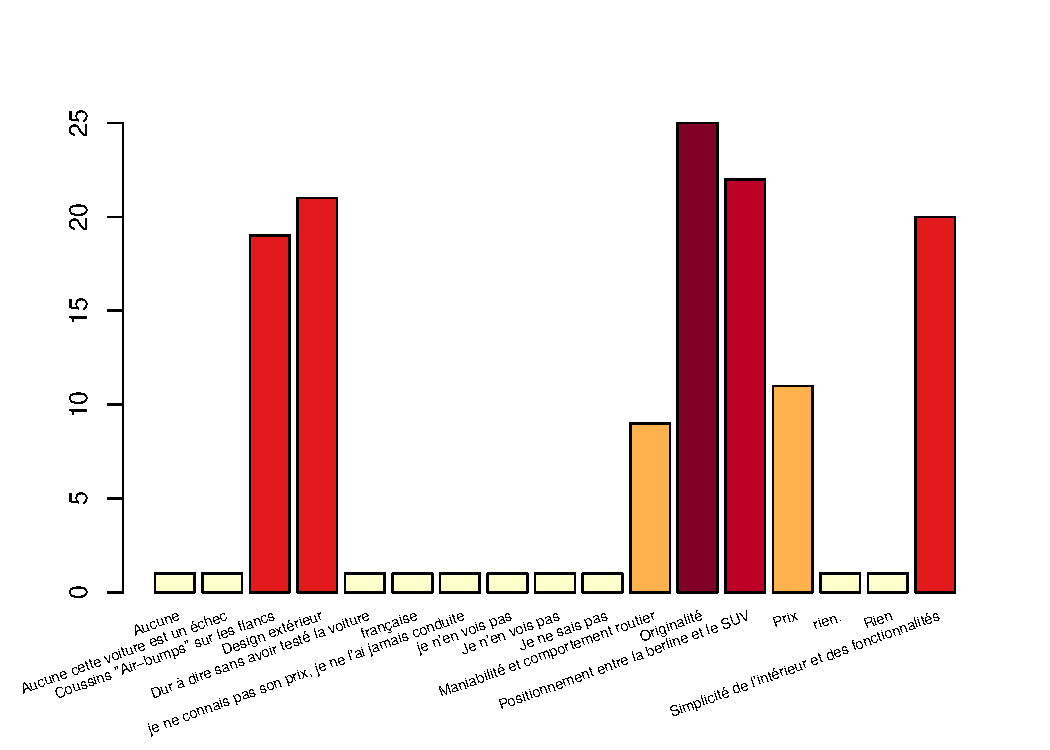
\includegraphics[width=\maxwidth]{figure/qualities_fr-1} \caption[Qualités de la C4 Cactus selon les personnes ayant répondu au sondage français]{Qualités de la C4 Cactus selon les personnes ayant répondu au sondage français}\label{fig:qualities fr}
\end{figure}


\end{knitrout}

\begin{knitrout}
\definecolor{shadecolor}{rgb}{0.969, 0.969, 0.969}\color{fgcolor}\begin{figure}[H]
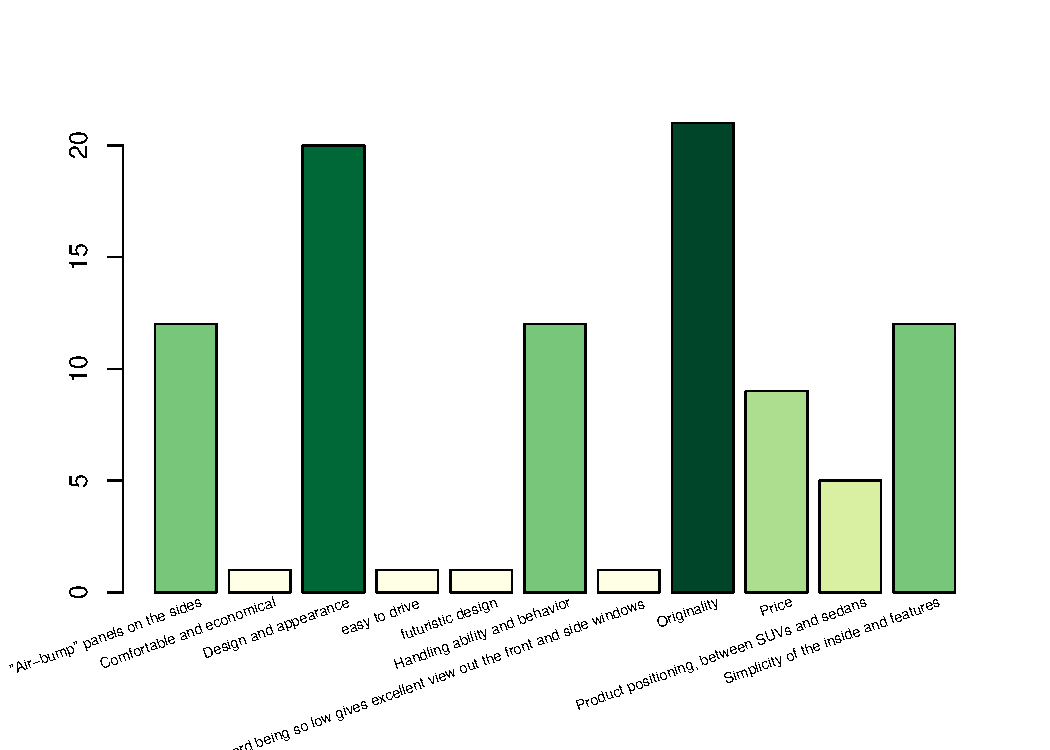
\includegraphics[width=\maxwidth]{figure/qualities_en-1} \caption[Qualités de la C4 Cactus selon les personnes ayant répondu au sondage anglais]{Qualités de la C4 Cactus selon les personnes ayant répondu au sondage anglais}\label{fig:qualities en}
\end{figure}


\end{knitrout}

\begin{knitrout}
\definecolor{shadecolor}{rgb}{0.969, 0.969, 0.969}\color{fgcolor}\begin{figure}[H]
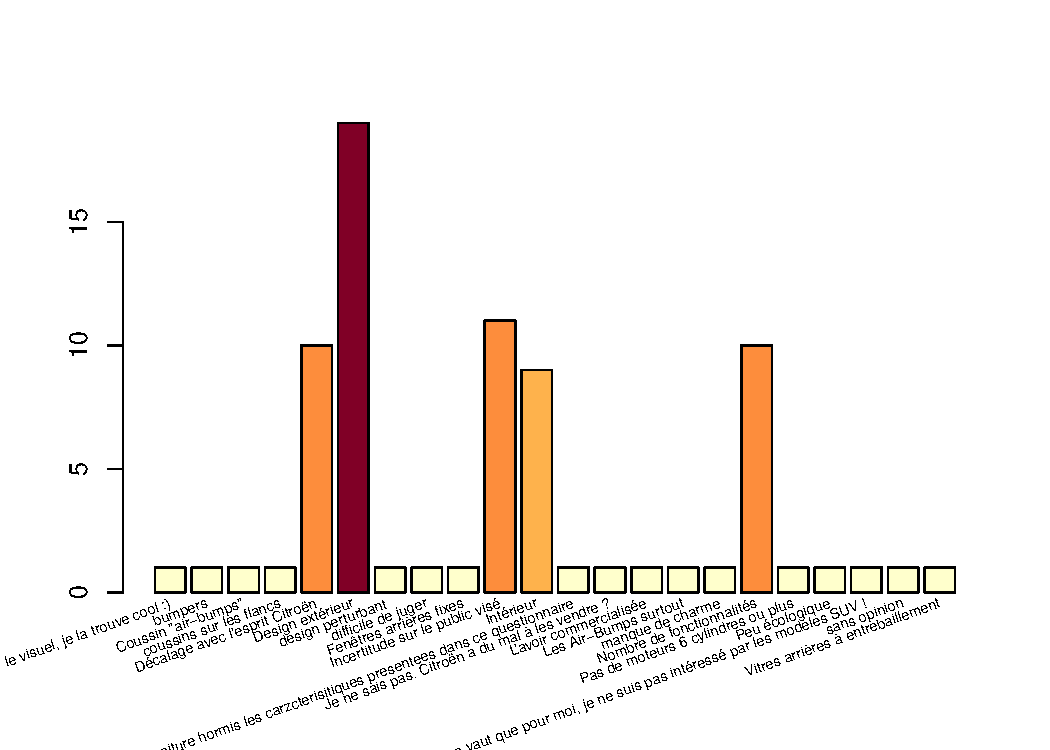
\includegraphics[width=\maxwidth]{figure/flaws_fr-1} \caption[Défauts de la C4 Cactus selon les personnes ayant répondu au sondage français]{Défauts de la C4 Cactus selon les personnes ayant répondu au sondage français}\label{fig:flaws fr}
\end{figure}


\end{knitrout}

\begin{knitrout}
\definecolor{shadecolor}{rgb}{0.969, 0.969, 0.969}\color{fgcolor}\begin{figure}[H]
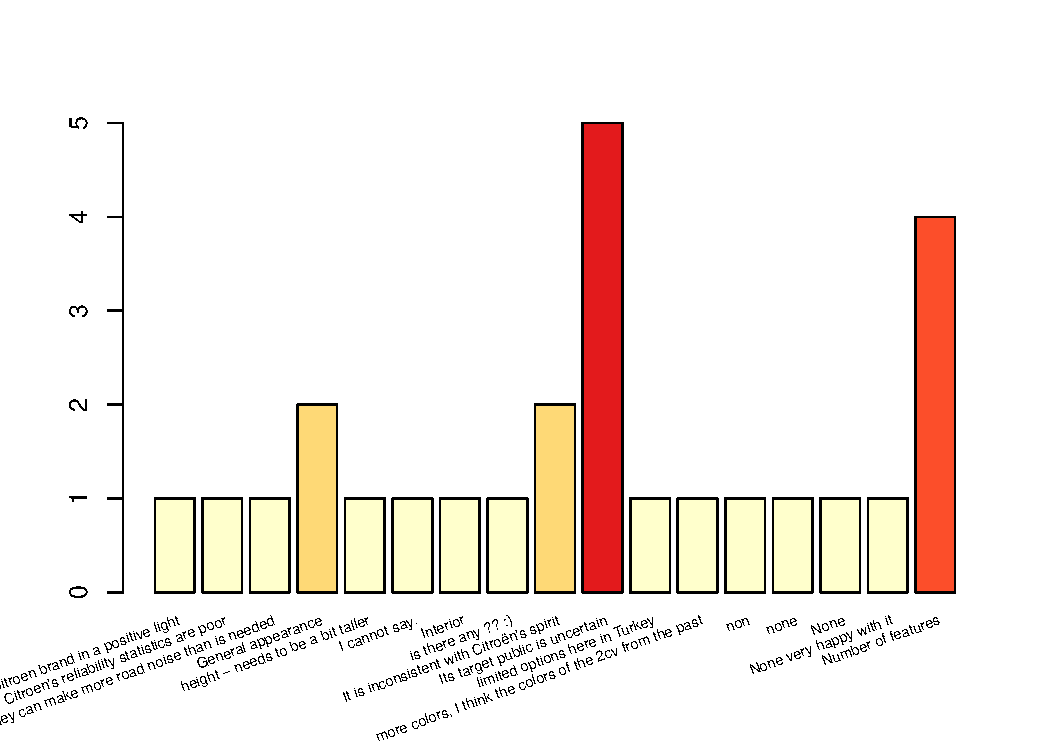
\includegraphics[width=\maxwidth]{figure/flaws_en-1} \caption[Défauts de la C4 Cactus selon les personnes ayant répondu au sondage anglais]{Défauts de la C4 Cactus selon les personnes ayant répondu au sondage anglais}\label{fig:flaws en}
\end{figure}


\end{knitrout}

\begin{knitrout}
\definecolor{shadecolor}{rgb}{0.969, 0.969, 0.969}\color{fgcolor}\begin{figure}[H]
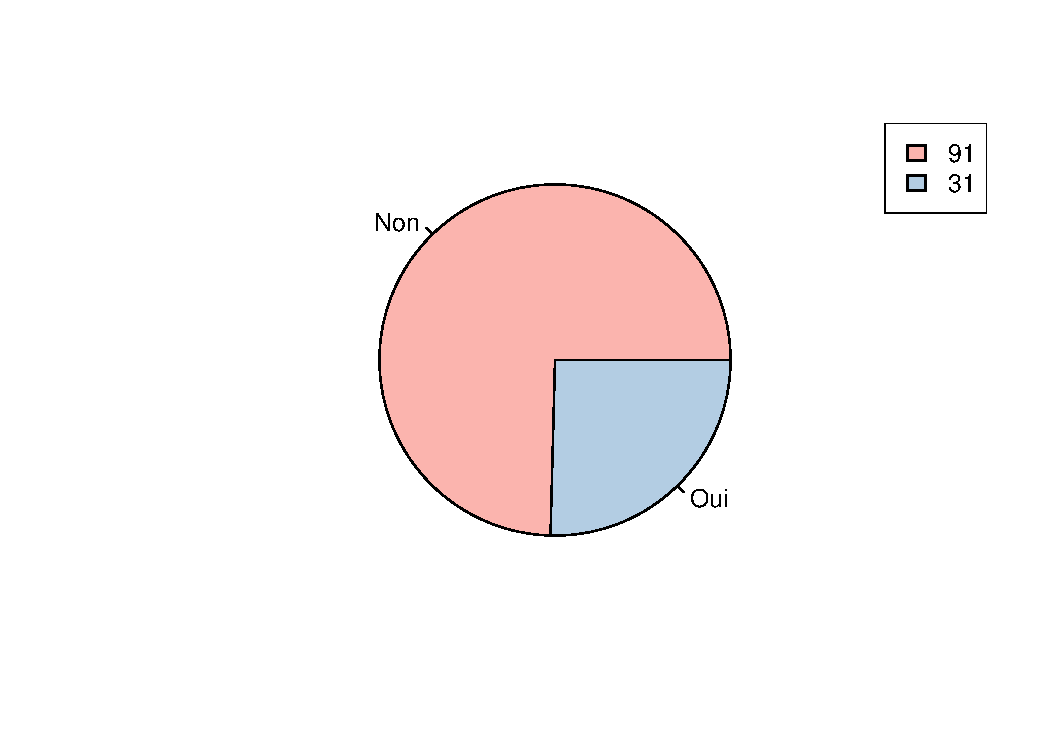
\includegraphics[width=\maxwidth]{figure/buy_fr-1} \caption[Proportion personnes ayant répondu au sondage français qui achèteraient une C4 Cactus]{Proportion personnes ayant répondu au sondage français qui achèteraient une C4 Cactus}\label{fig:buy fr}
\end{figure}


\end{knitrout}

\begin{knitrout}
\definecolor{shadecolor}{rgb}{0.969, 0.969, 0.969}\color{fgcolor}\begin{figure}[H]
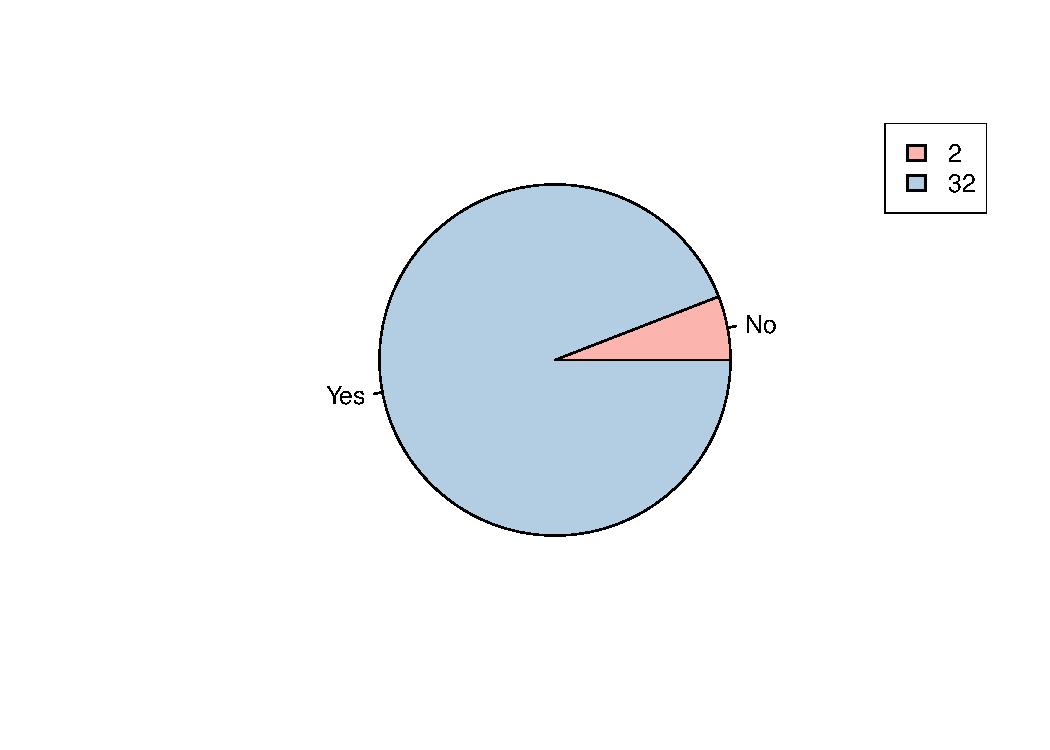
\includegraphics[width=\maxwidth]{figure/buy_en-1} \caption[Proportion personnes ayant répondu au sondage anglais qui achèteraient une C4 Cactus]{Proportion personnes ayant répondu au sondage anglais qui achèteraient une C4 Cactus}\label{fig:buy en}
\end{figure}


\end{knitrout}

\section{La marque DS}

\begin{knitrout}
\definecolor{shadecolor}{rgb}{0.969, 0.969, 0.969}\color{fgcolor}\begin{figure}[H]
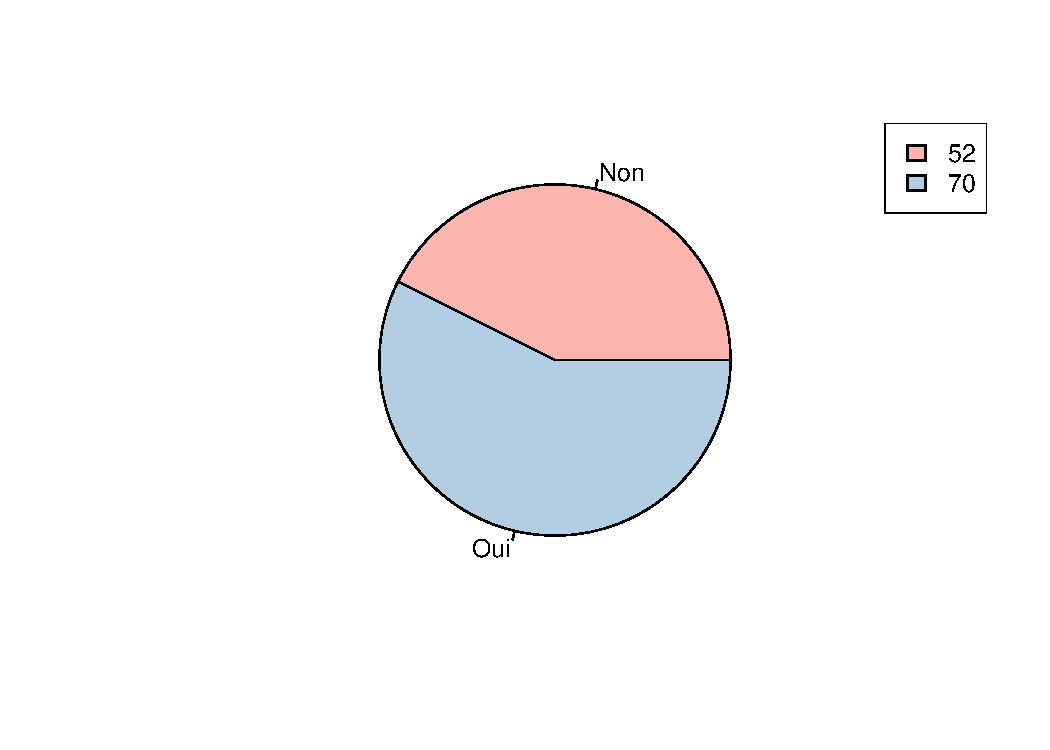
\includegraphics[width=\maxwidth]{figure/ds_know_fr-1} \caption[Proportion personnes ayant répondu au sondage français sachant que DS était une marque indépendante]{Proportion personnes ayant répondu au sondage français sachant que DS était une marque indépendante}\label{fig:ds know fr}
\end{figure}


\end{knitrout}

\begin{knitrout}
\definecolor{shadecolor}{rgb}{0.969, 0.969, 0.969}\color{fgcolor}\begin{figure}[H]
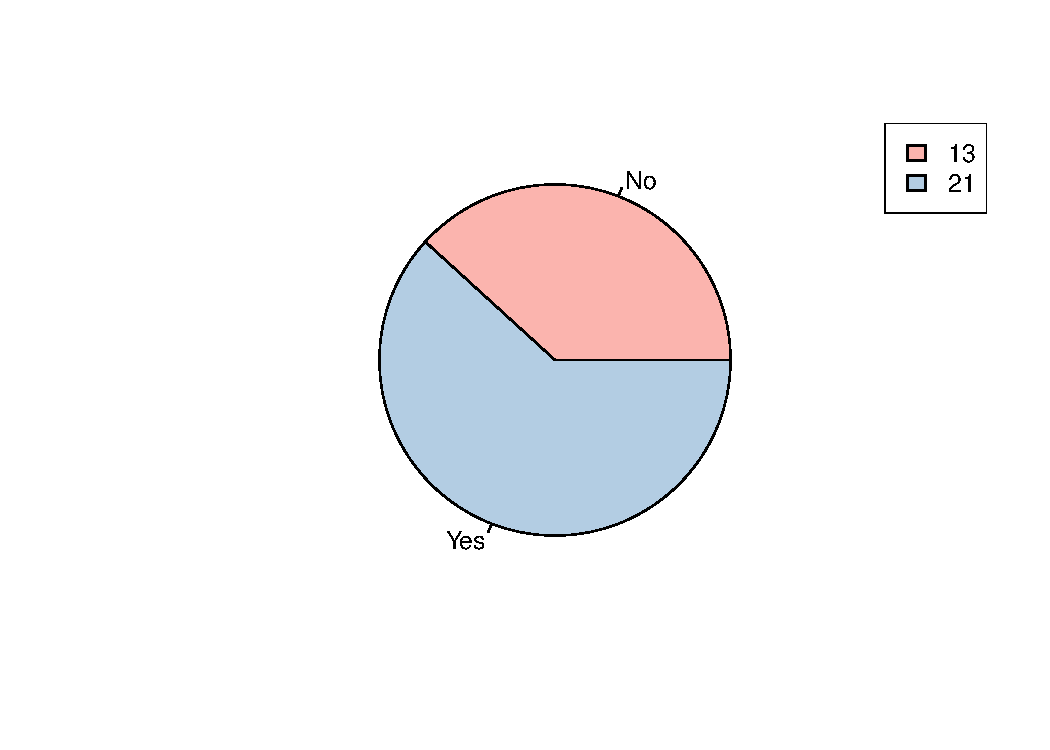
\includegraphics[width=\maxwidth]{figure/ds_know_en-1} \caption[Proportion personnes ayant répondu au sondage anglais sachant que DS était une marque indépendante]{Proportion personnes ayant répondu au sondage anglais sachant que DS était une marque indépendante}\label{fig:ds know en}
\end{figure}


\end{knitrout}

\begin{knitrout}
\definecolor{shadecolor}{rgb}{0.969, 0.969, 0.969}\color{fgcolor}\begin{figure}[H]
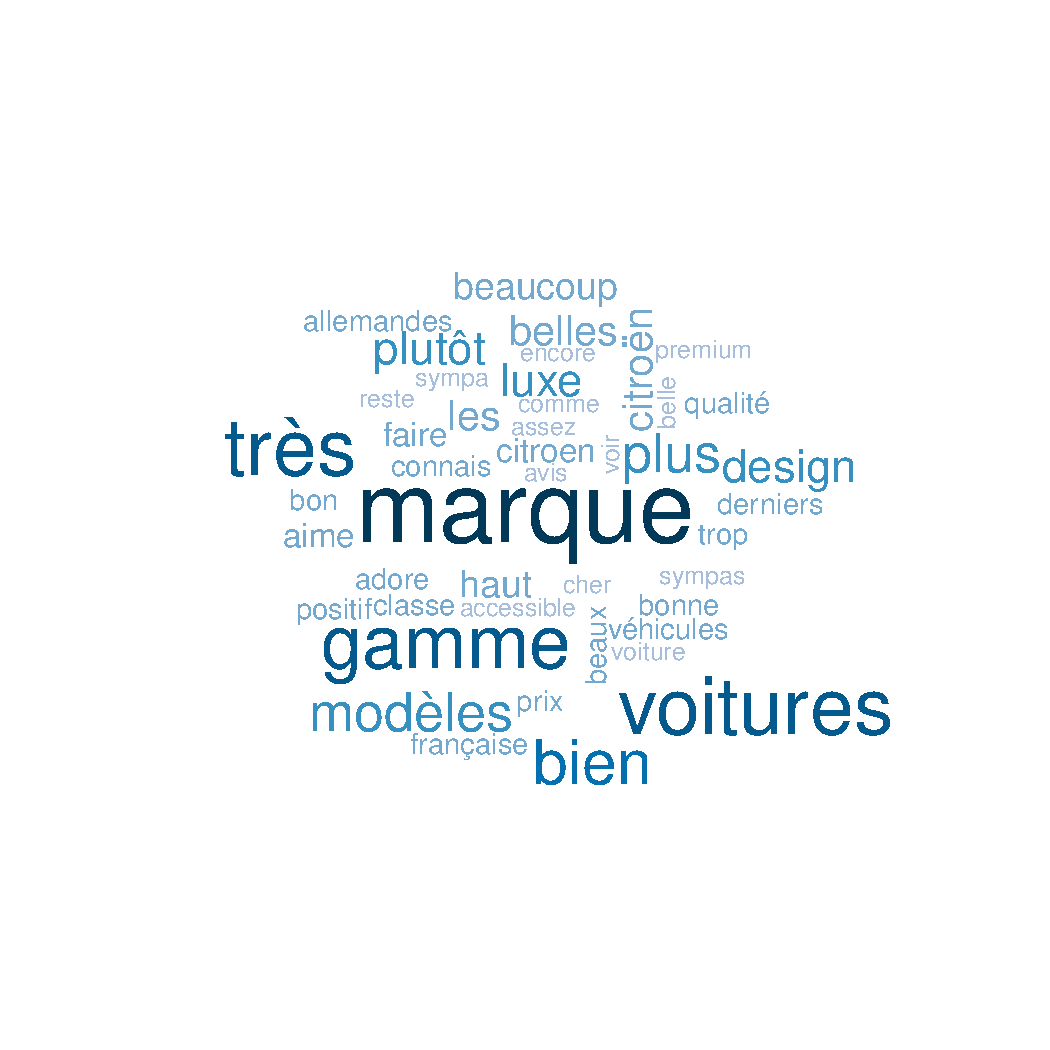
\includegraphics[width=\maxwidth]{figure/brand_fr-1} \caption[Nuage de mots de l'avis de la marque DS des personnes ayant répondu au sondage français]{Nuage de mots de l'avis de la marque DS des personnes ayant répondu au sondage français}\label{fig:brand fr}
\end{figure}


\end{knitrout}

\begin{knitrout}
\definecolor{shadecolor}{rgb}{0.969, 0.969, 0.969}\color{fgcolor}\begin{figure}[H]
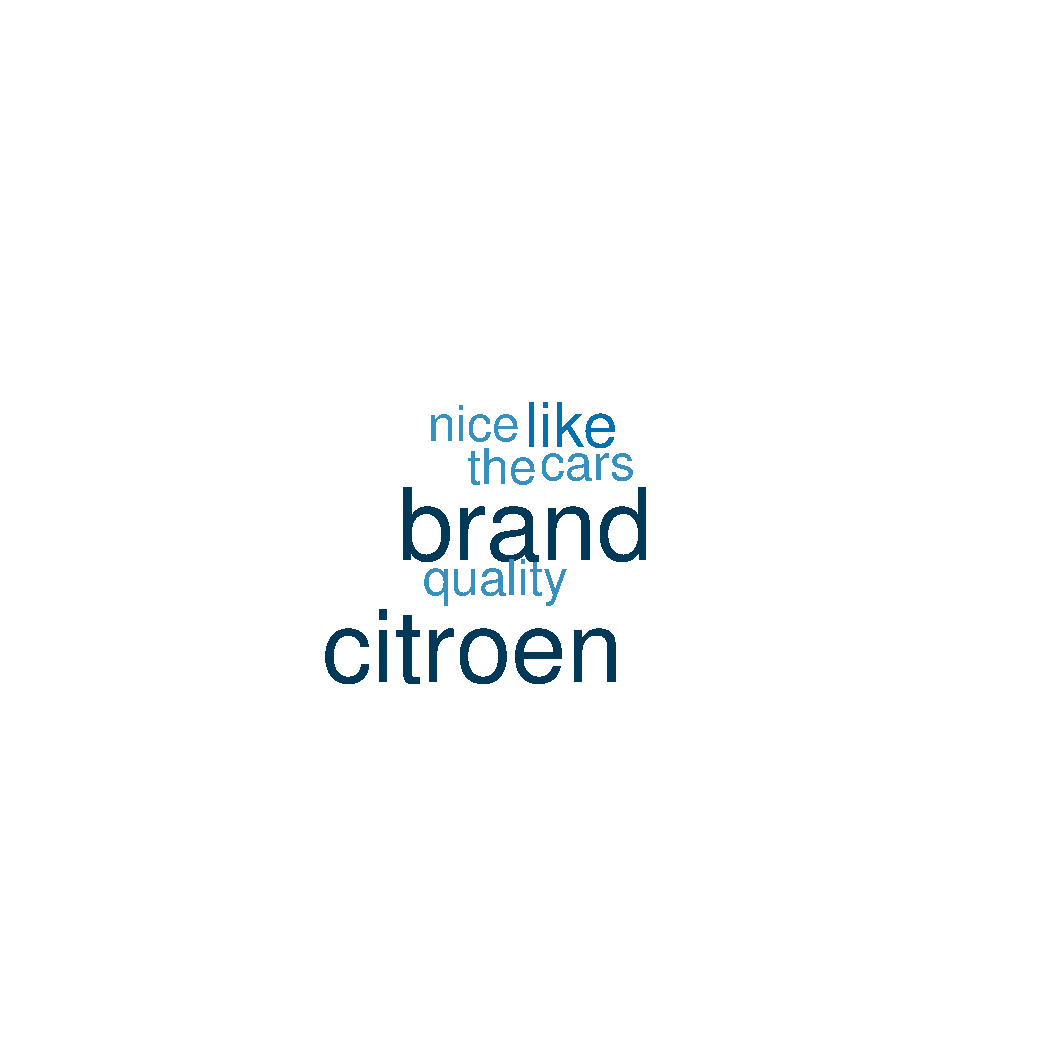
\includegraphics[width=\maxwidth]{figure/brand_en-1} \caption[Nuage de mots de l'avis de la marque DS des personnes ayant répondu au sondage anglais]{Nuage de mots de l'avis de la marque DS des personnes ayant répondu au sondage anglais}\label{fig:brand en}
\end{figure}


\end{knitrout}

\begin{knitrout}
\definecolor{shadecolor}{rgb}{0.969, 0.969, 0.969}\color{fgcolor}\begin{figure}[H]
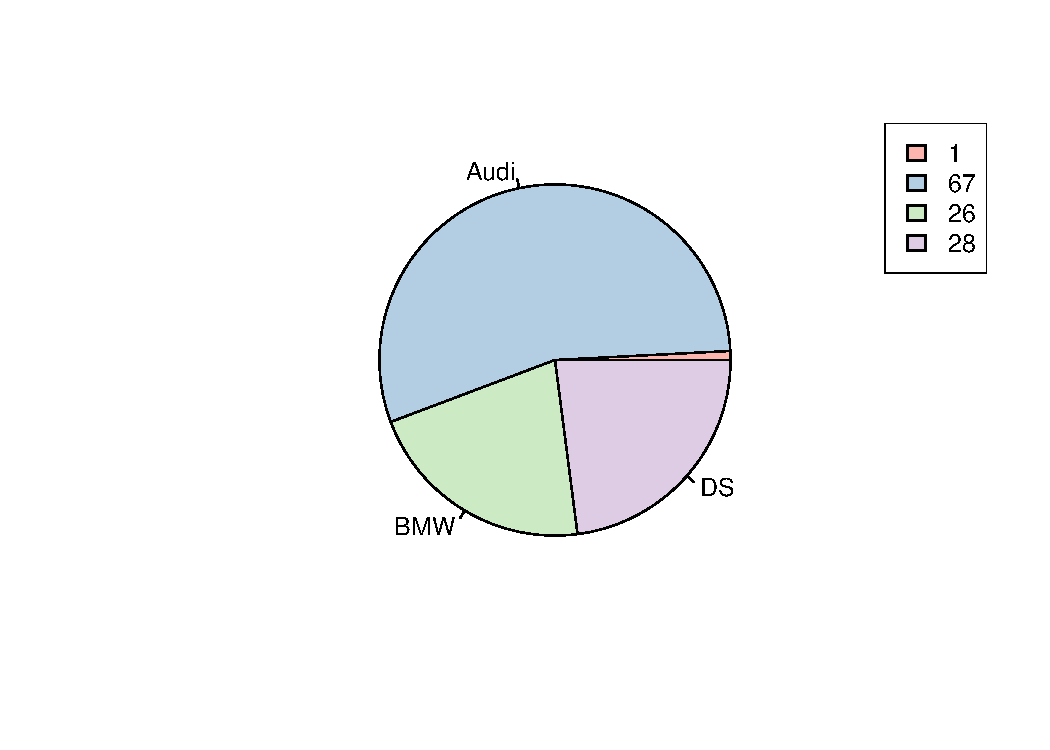
\includegraphics[width=\maxwidth]{figure/preference_fr-1} \caption[Préférences de marque des personnes ayant répondu au sondage français]{Préférences de marque des personnes ayant répondu au sondage français}\label{fig:preference fr}
\end{figure}


\end{knitrout}

\begin{knitrout}
\definecolor{shadecolor}{rgb}{0.969, 0.969, 0.969}\color{fgcolor}\begin{figure}[H]
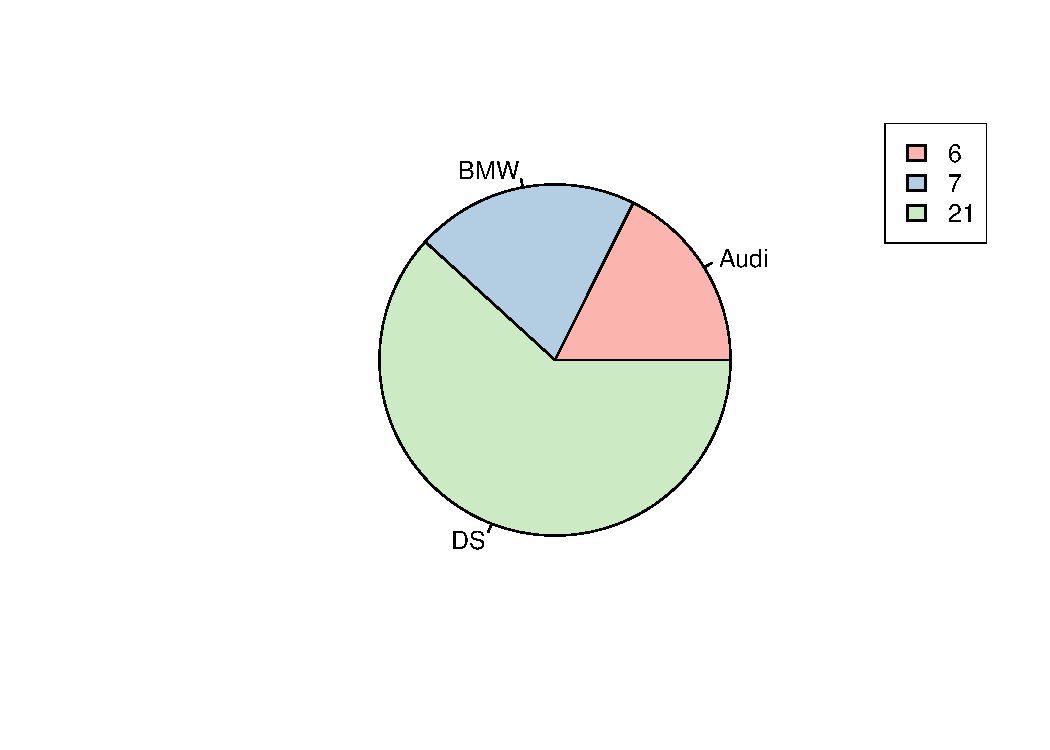
\includegraphics[width=\maxwidth]{figure/preference_en-1} \caption[Préférences de marque des personnes ayant répondu au sondage anglais]{Préférences de marque des personnes ayant répondu au sondage anglais}\label{fig:preference en}
\end{figure}


\end{knitrout}

\begin{knitrout}
\definecolor{shadecolor}{rgb}{0.969, 0.969, 0.969}\color{fgcolor}\begin{figure}[H]
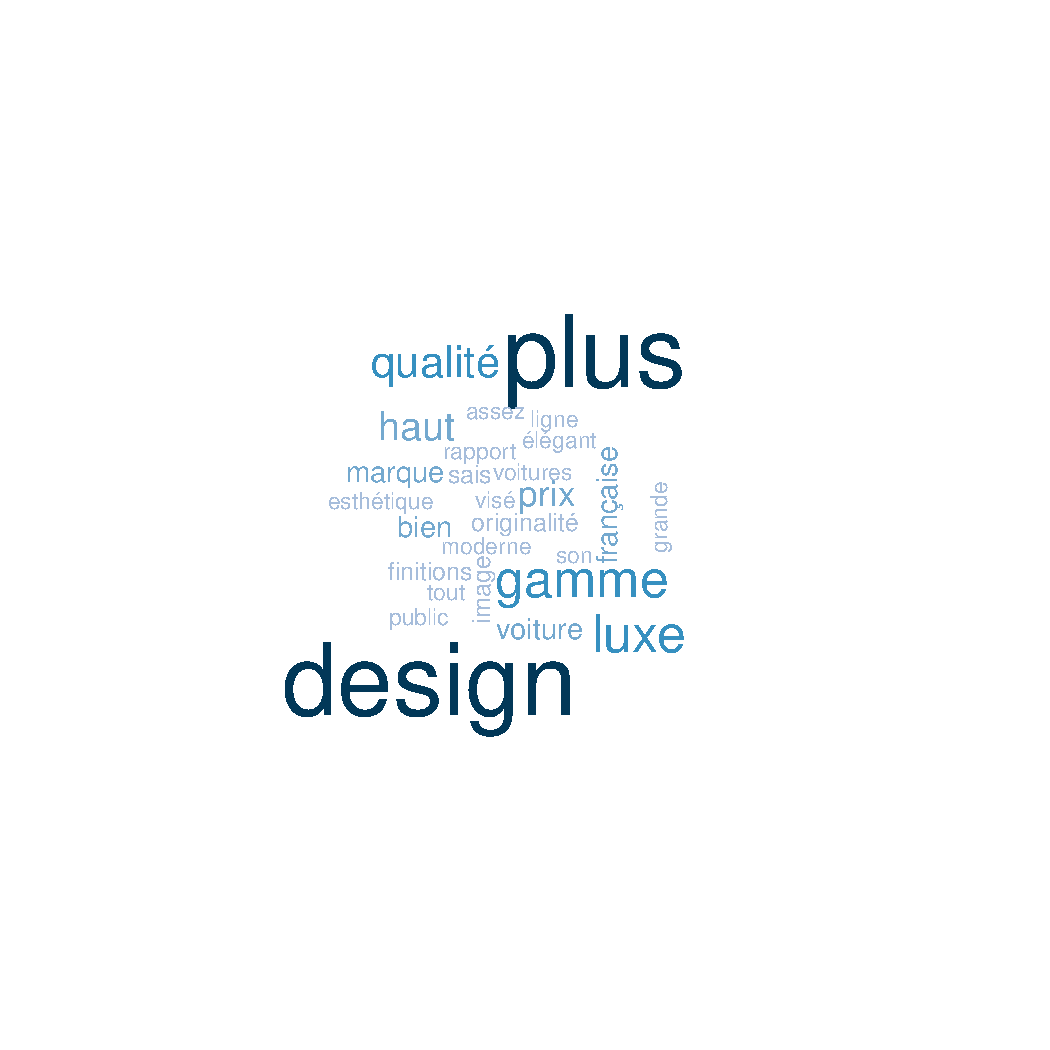
\includegraphics[width=\maxwidth]{figure/differences_fr-1} \caption[Nuage de mots de l'avis de la marque DS des personnes ayant répondu au sondage français]{Nuage de mots de l'avis de la marque DS des personnes ayant répondu au sondage français}\label{fig:differences fr}
\end{figure}


\end{knitrout}

\begin{knitrout}
\definecolor{shadecolor}{rgb}{0.969, 0.969, 0.969}\color{fgcolor}\begin{figure}[H]
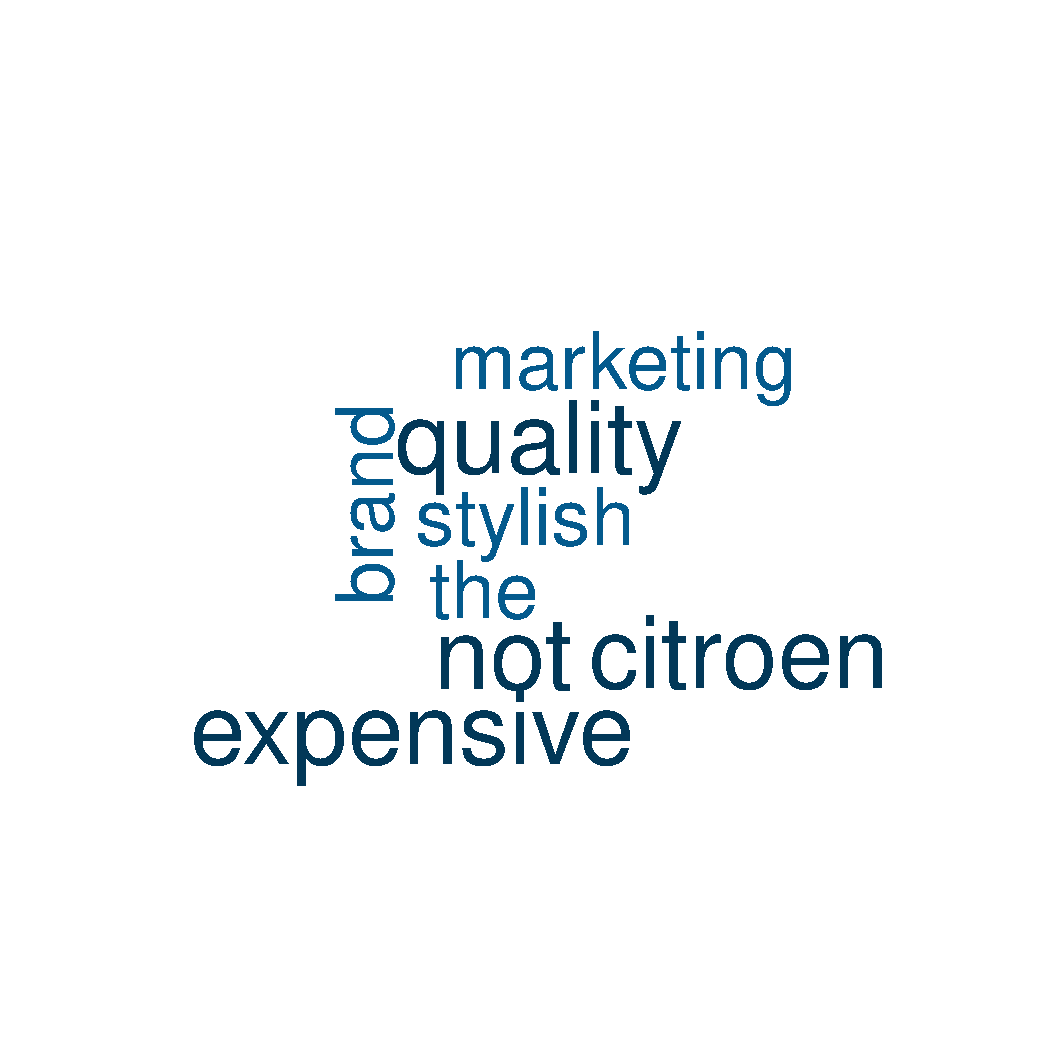
\includegraphics[width=\maxwidth]{figure/differences_en-1} \caption[Nuage de mots de l'avis de la marque DS des personnes ayant répondu au sondage anglais]{Nuage de mots de l'avis de la marque DS des personnes ayant répondu au sondage anglais}\label{fig:differences en}
\end{figure}


\end{knitrout}

\printbibliography%

\end{document}

% vim: spell : spelllang=fr
